\documentclass{article}
\usepackage{amsmath, amssymb, amsfonts, amsthm, mathtools, bm}
\usepackage{color,comment}
\usepackage{geometry}
\usepackage{hyperref}
\usepackage[english]{babel}
\usepackage{graphicx}
% \usepackage{biblatex}
% \addbibresource{bibliography.bib}

\title{Blending SIR and Predator-Prey Models to Predict the Labor Market}

\author{Jason Vasquez \and Dylan Skinner \and Benjamin Mcmullin \and Ethan Crawford}

\date{December 5 2023}

\begin{document}

\maketitle

We give permission for this work to be shared by ACME Volume 4 instructors and anybody else who may have reasonable motivation.

\begin{abstract}

The labor market, including the unemployment rate and the amount of workers looking for jobs, can have a large impact on the economny.
The more people employed means more money being spent, which in turn means more money being made. 
Furthermore, rise in unemployment can lead to a recession. Being able to predict the labor market can help us prepare for a recession and help us understand the economy better.
In this paper, we adapt an SIR model to model the amount of employed, unemployed, and retired individuals.
Furthermore, we use a quasi predator-prey model to illustrate the oscillation of the two industries commonly known as white-collar and blue-collar.

\end{abstract}

\section{Background/Motivation}

One thing that is certain in life is that people will always need jobs. Not only this, but people 
will often lose their jobs. Not only this, but people will (eventually) retire from their jobs.
The focus of our project is modeling this situation.

Our investigation navigates the intricate dynamics of employment trajectories and occupational sectors. 
Employing the SIR (Susceptible-Infectious-Recovered) model, typically used for disease dynamics but adapted 
here to study employment dynamics, we aim to comprehend the propagation of employment statuses—specifically, 
the transitions between being employed, unemployed, and retired. A discernible trend has emerged in recent times, 
notably influenced by the technological revolution. The surge in interest and demand for tech-oriented careers 
has prompted a significant shift away from traditional blue-collar professions. This migration has led to a 
dual challenge: a scarcity of skilled workers in the blue-collar sector and an oversaturation of the tech 
industry. Our study extends beyond the conventional SIR model, incorporating elements of a quasi-predator-prey 
framework inspired by ecological models. This approach allows us to capture the nuanced relationship between 
the blue-collar and white-collar industries, offering insights into the cyclical dynamics between these sectors. 
Motivated by the imperative to comprehend and address the consequences of this evolving employment landscape, 
our research aims to contribute valuable insights for informing strategic policies and industry interventions.

\section{Modeling}

\subsection{Labor Force, Unemployed, and Retired}

We begin by building off the work of (cite ElFalidy). In their work, ElFadily et. al. proposed a model
 representing the labor force and unemployed populations. They begin by defining their equations as

\begin{align}
    \begin{split}
        \frac{dL}{dt} &= \gamma U - (\sigma + \mu)L, \\
        \frac{dU}{dt} &= \rho \left(1 - \frac{L_{\tau} + U_{\tau}}{N_c} \right)L_{\tau} + \sigma L - (\gamma + \mu)U, \\
    \end{split}
\end{align}

where $L$ is the labor force, $U$ is the unemployed population, with initial conditions for (1) defined as:

\begin{align}
    \begin{split}
        L(0) &> 0 , \\
        U(0) &> 0, \\
        (L(\theta),U(\theta)) &= (\varphi_1(\theta), \varphi_2(\theta)), \quad \theta \in [-\tau,0], \\
    \end{split}
\end{align}
where $\varphi_i\in C([-\tau, 0], \mathbb{R}^+),\;\; i=1,2$.

The parameters are defined as follows:

\begin{itemize}
    \item $\gamma$: employment rate
    \item $\sigma$: rate of job loss 
    \item $\mu$: mortality rate
    \item $\rho$: maximum population growth rate 
    \item $N_c$: population carrying capacity 
    \item $\tau$: time lag needed to contribute in the reproductive process of a new individual looking for a job
\end{itemize}
 

With this information in mind, we can begin to adapt this model to fit our needs. We begin by adding a third population, the retired population, $R$.
We can then define our new equations as

\begin{align}
    \begin{split}
        \frac{dL}{dt} &= \gamma U - (\sigma + \mu)L {\color{red}\;- \left(\frac{\Sigma}{L_{\tau} + U_{\tau}}\right) L + \omega\left(\frac{\Sigma}{L_{\tau} + U_{\tau}}\right) R},\\
        \frac{dU}{dt} &= \rho\left(1 - \frac{L_{\tau} + U_{\tau}}{N_c} \right)L_{\tau} + \sigma L -(\mu + \gamma)U,  \\
        \frac{dR}{dt} &= {\color{red}\left(\frac{\Sigma}{L_{\tau} + U_{\tau}}\right) L - \omega\left(\frac{\Sigma}{L_{\tau} + U_{\tau}}\right) R \; - \, \mu R},
    \end{split}
\end{align}

which simplify to 

\begin{align}
    \begin{split}
        \frac{dL}{dt} &= \gamma U - (\sigma + \mu)L {\color{red}\; + \;(\omega R - L)\left(\frac{\Sigma}{L + U}\right)},\\
        \frac{dU}{dt} &= \rho\left(1 - \frac{L + U}{N_c} \right)L_{\tau} + \sigma L -(\mu + \gamma)U  \\
        \frac{dR}{dt} &= {\color{red}(L - \omega R)\left(\frac{\Sigma}{L + U}\right) \; - \, \mu R}.
    \end{split}
\end{align}

One of the first things to note from our equations is the removal of the time lag $\tau$. 
This is because, instead of factoring in people when they are bor, we are instead factoring them
in when they turn of working age (16). This reduces unnecessary complexity in our model. Another thing to note
is that we have added two new parameters, $\omega$ and $\Sigma$. We define $\Sigma$ to be the number of people who
retire each year in the United States, and $\omega$ to be the rate at which retired people enter back
into the full-time workforce. We can then define our new initial conditions as:

\begin{align}
    \begin{split}
        L(0) &> 0 , \\
        U(0) &> 0, \\
        R(0) &> 0, \\
        (L(\theta),U(\theta), R(\theta)) &= (\varphi_1(\theta), \varphi_2(\theta), \varphi_3(\theta)), \quad \theta \in [-\tau,0], \\
    \end{split}
\end{align}
where $\varphi_i\in C([-\tau, 0], \mathbb{R}^+),\;\; i=1,2,3$.







\section{Related Work}

Here is a cool graph. Please accept it as nothing but the truth. This is a change!

\begin{figure}[h]
    \centering
    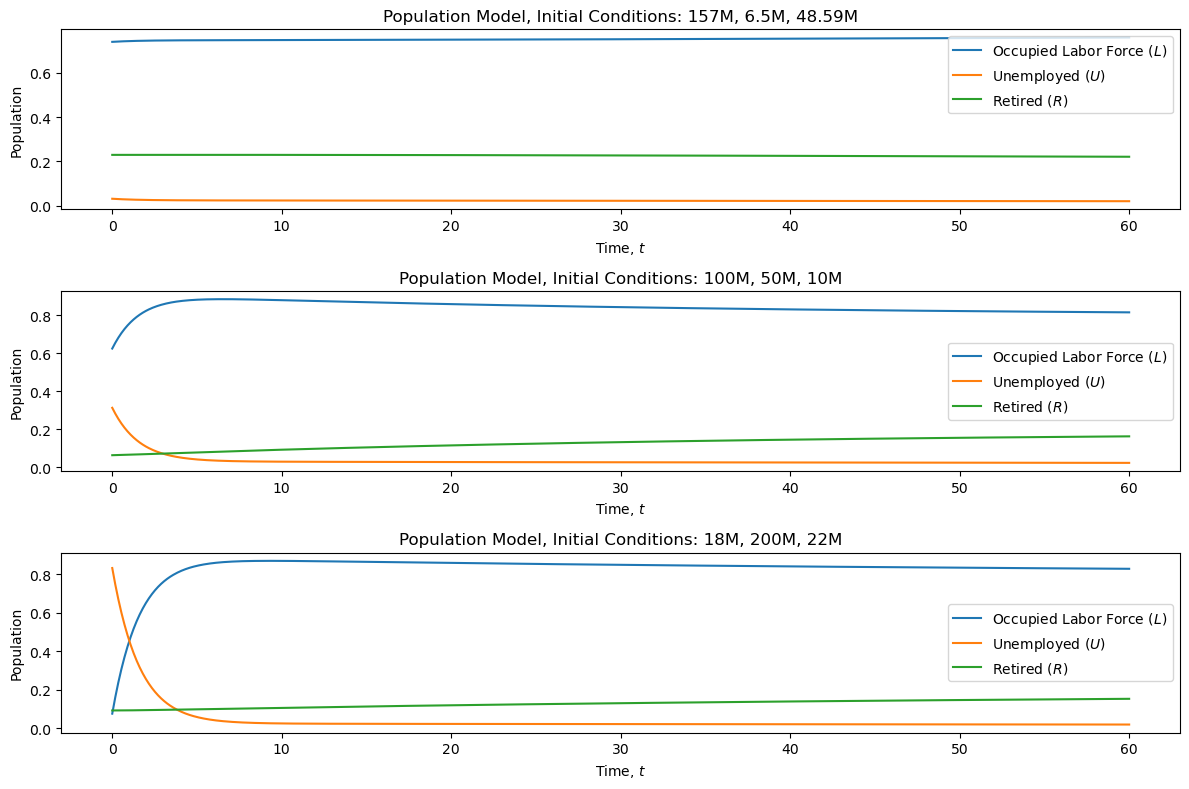
\includegraphics[width=\textwidth]{figures/vol4_proj_pic.png}
    \caption{A cool graph}
    \label{fig:cool_graph}
\end{figure}

% Rest of your document goes here
% \printbibliography


\end{document}
